\chapter{Measurement Results}
\label{ch_results}

As discussed in Section \ref{sec_applying_method}, we applied our method to the MI domain. This section shows the summary of the measurement results. The detailed data can be found in the repository \hyperlink{https://data.mendeley.com/datasets/k3pcdvdzj2/1}{https://data.mendeley.com/datasets/k3pcdvdzj2/1}.

Table \ref{tab_final_list} shows the 29 software packages that we measured. We found the initial release dates (Rlsd) in their documents for most projects and marked the rest two with ``?". We used the date of the latest change to each code repository to decide the latest update. We found out funding information (Fnd) for only eight projects.

We counted the number of contributors (NOC) and lines of code (LOC). we considered anyone who made at least one accepted commit to the source code as a contributor. Thus, it does not mean that any development team has are 100 long-term members. Many of these projects received change requests and code from the community, such as pull requests and git commits on GitHub.

Table \ref{tab_final_list} also shows the supported OS for each software package, and 25 of them could work on all three Windows (W), macOS (M), and Linux (L) systems. However, there was a significant difference in the philosophy to achieve cross-platform compatibility. Most of them were native software products, but five were naturally platform-independent web applications.

\begin{table}[H]
\begin{tabular}{llllllllll}
\hline
\multirow{2}{*}{Software} & \multirow{2}{*}{Rlsd} & \multirow{2}{*}{Updated} & \multirow{2}{*}{Fnd} & \multirow{2}{*}{NOC} & \multirow{2}{*}{LOC} & \multicolumn{3}{c}{OS} & \multirow{2}{*}{W} \\ \cline{7-9}
 &  &  &  &  &  & W & M & L &  \\ \hline
3D Slicer \cite{Kikinis2014} & 1998 & 2020-08 & X & 100 & 501451 & X & X & X &  \\
Ginkgo CADx \cite{Wollny2020} & 2010 & 2019-05 &  & 3 & 257144 & X & X & X &  \\
XMedCon \cite{Nolf2003} & 2000 & 2020-08 &  & 2 & 96767 & X & X & X &  \\
Weasis \cite{Roduit2021} & 2010 & 2020-08 &  & 8 & 123272 & X & X & X &  \\
MRIcroGL \cite{Rorden2021} & 2015 & 2020-08 &  & 2 & 8493 & X & X & X &  \\
SMILI \cite{Chandra2018} & 2014 & 2020-06 &  & 9 & 62626 & X & X & X &  \\
ImageJ \cite{Rueden2017} & 1997 & 2020-08 & X & 18 & 9681 & X & X & X &  \\
Fiji \cite{Schindelin2012} & 2011 & 2020-08 & X & 55 & 10833 & X & X & X &  \\
DicomBrowser \cite{Archie2012} & 2012 & 2020-08 &  & 3 & 5505 & X & X & X &  \\
3DimViewer \cite{TESCAN2020} & ? & 2020-03 & X & 3 & 178065 & X & X &  &  \\
Horos \cite{horosproject2020} & ? & 2020-04 &  & 21 & 561617 &  & X &  &  \\
OsiriX Lite \cite{PixmeoSARL2019} & 2004 & 2019-11 &  & 9 & 544304 &  & X &  &  \\
dwv \cite{Martelli2021} & 2012 & 2020-09 &  & 22 & 47815 & X & X & X & X \\
Drishti \cite{Limaye2012} & 2012 & 2020-08 &  & 1 & 268168 & X & X & X &  \\
\begin{tabular}[c]{@{}l@{}}BioImage Suite\\ Web \cite{Papademetris2005}\end{tabular} & 2018 & 2020-10 & X & 13 & 139699 & X & X & X & X \\
OHIF Viewer \cite{Ziegler2020} & 2015 & 2020-10 &  & 76 & 63951 & X & X & X & X \\
Slice:Drop \cite{Haehn2013} & 2012 & 2020-04 &  & 3 & 19020 & X & X & X & X \\
GATE \cite{Jan2004} & 2011 & 2020-10 &  & 45 & 207122 &  & X & X &  \\
ITK-SNAP \cite{Yushkevich2006} & 2006 & 2020-06 & X & 13 & 88530 & X & X & X &  \\
ParaView \cite{Ahrens2005} & 2002 & 2020-10 & X & 100 & 886326 & X & X & X & X \\
MatrixUser \cite{Liu2016} & 2013 & 2018-07 &  & 1 & 23121 & X & X & X &  \\
\end{tabular}
\end{table}

\begin{table}[H]
\begin{tabular}{llllllllll}
\hline
\multirow{2}{*}{Software} & \multirow{2}{*}{Rlsd} & \multirow{2}{*}{Updated} & \multirow{2}{*}{Fnd} & \multirow{2}{*}{NOC} & \multirow{2}{*}{LOC} & \multicolumn{3}{c}{OS} & \multirow{2}{*}{W} \\ \cline{7-9}
 &  &  &  &  &  & W & M & L &  \\ \hline
DICOM Viewer \cite{Afsar2021} & 2018 & 2020-04 & X & 5 & 30761 & X & X & X &  \\
INVESALIUS 3 \cite{Amorim2015} & 2009 & 2020-09 &  & 10 & 48605 & X & X & X &  \\
medInria \cite{Fillard2012} & 2009 & 2020-11 &  & 21 & 148924 & X & X & X &  \\
dicompyler \cite{Panchal2010} & 2009 & 2020-01 &  & 2 & 15941 & X & X &  &  \\
MicroView \cite{ParallaxInnovations2020} & 2015 & 2020-08 &  & 2 & 27470 & X & X & X &  \\
Papaya \cite{UTHSCSA2019} & 2012 & 2019-05 &  & 9 & 71831 & X & X & X &  \\
AMIDE \cite{Loening2017} & 2006 & 2017-01 &  & 4 & 102827 & X & X & X &  \\
Gwyddion \cite{Nevcas2012} & 2004 & 2020-11 &  & 38 & 643427 & X & X & X &  \\ \hline
\end{tabular}
\caption{\label{tab_final_list}Final software list}
\end{table}

Most of the projects used more than one programming language, including a primary language that the developers used the most. Figure \ref{fig_language} shows the primary languages versus the number of projects using them.

\begin{figure}[H]
\centering
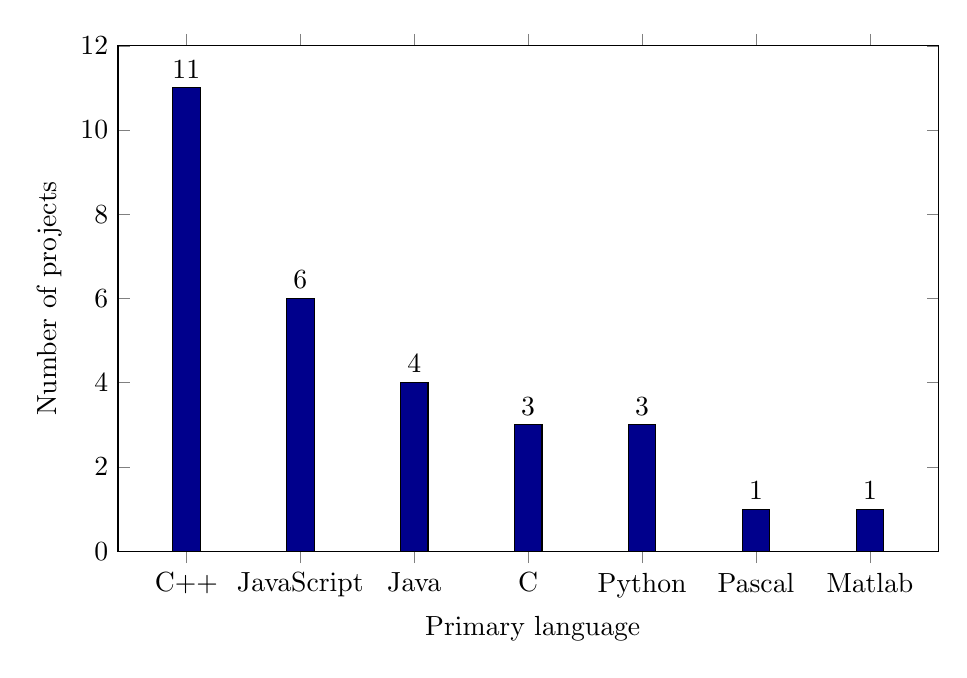
\begin{tikzpicture}
\centering
\begin{axis}
[
ybar,
height=8cm,
width=12cm,
ylabel={Number of projects},
xlabel={\ Primary language},
symbolic x coords={C++, JavaScript, Java, C, Python, Pascal, Matlab},
xtick=data,
nodes near coords,
nodes near coords align={vertical},
]
\addplot[black,fill=blue!55!black] coordinates {(C++,11) (JavaScript,6) (Java,4) (C,3) (Python,3) (Pascal,1) (Matlab,1) };
\end{axis}  
\end{tikzpicture}
\caption{\label{fig_language}Primary languages versus number of projects using them}
\end{figure}

We failed installing \textit{DICOM Viewer}, so we could not test \textit{surface reliability} and \textit{surface robustness} for it. We kept this software on our list because the other seven qualities do not rely on a successful installation. Besides, it used a unique dependency, and we wanted to keep the diversity.

\section{Installability}
\label{sec_result_installability}

Figure \ref{fg_installability_scores} lists the scores of \textit{installability}.

\begin{figure}[H]
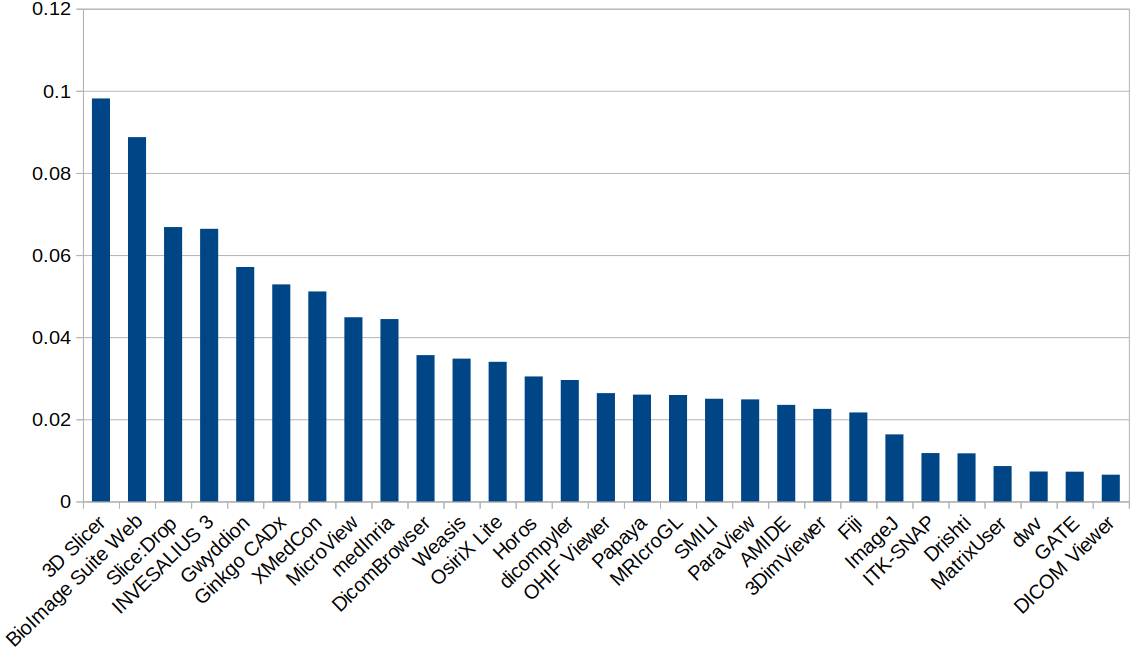
\includegraphics[scale=0.38]{figures/installability_scores.png}
\caption{AHP installability scores}
\label{fg_installability_scores}
\end{figure}

We found installation instructions for 16 projects. Among the ones without such an instruction, \textit{BioImage Suite Web} and \textit{Slice:Drop} were web applications and provided online versions to use, thus they needed no installation. Installing 10 of the projects needed extra dependencies. Five of them are the web applications in Table \ref{tab_final_list}, and depended on a browser; \textit{dwv}, \textit{OHIF Viewer}, and \textit{GATE} needed extra dependencies to build; \textit{ImageJ} and	\textit{Fiji} needed an unzip tool; \textit{MatrixUser} was based on Matlab; \textit{DICOM Viewer} needed to work on Nextcloud platform.

\textit{3D Slicer} has the highest score because it had easy-to-follow installation instructions, and the installation processes were automated, fast, and frustration-free, with all dependencies automatically added. There were also no errors during the installation and uninstallation steps. Many other software packages also had installation instructions and automated installers, and we had no trouble installing them, such as \textit{INVESALIUS 3}, \textit{Gwyddion}, \textit{XMedCon}, and \textit{MicroView}. We gave them various scores based on the understandability of the instructions, installation steps, and user experience. Since \textit{BioImage Suite Web} and \textit{Slice:Drop} needed no installation, we gave them higher scores due to the significant convenience. \textit{BioImage Suite Web} also provided an option to download cache to local for offline usage, which was easy to apply.

\textit{dwv}, \textit{GATE}, and \textit{DICOM Viewer} showed severe problems. We could not install them due to some issues that we could not solve. We spent a reasonable amount of time on these problems, then considered them major obstacles for normal users if we still did not figure out any solutions. We suspect that only a part of the users faced the same problems, and given a lot of time, we might be able to find solutions. However, the difficulties greatly impacted the installation experiences, and we graded these software packages with lower scores. For example, \textit{dwv} and \textit{GATE} had the option to build from the source code, and we failed the building processes following the instructions. Although we could not locally build them, we could use a deployed online version for \textit{dwv}, and a VM version for \textit{GATE}. With those, we finished all the measurements for them. Furthermore, \textit{DICOM Viewer} depended on a cloud platform, and we could not successfully install the dependency.

\textit{MatrixUser} has a lower score because it depended on Matlab. We considered installing Matlab takes many more steps and time, and some users may not have a license to use Matlab.

\section{Correctness \& Verifiability}
The scores of \textit{correctness \& verifiability} are shown in Figure \ref{fg_correctness_erifiability_scores}. Generally speaking, the packages with higher scores adopted more techniques to improve \textit{correctness}, and had better documents for us to verify it.

\begin{figure}[H]
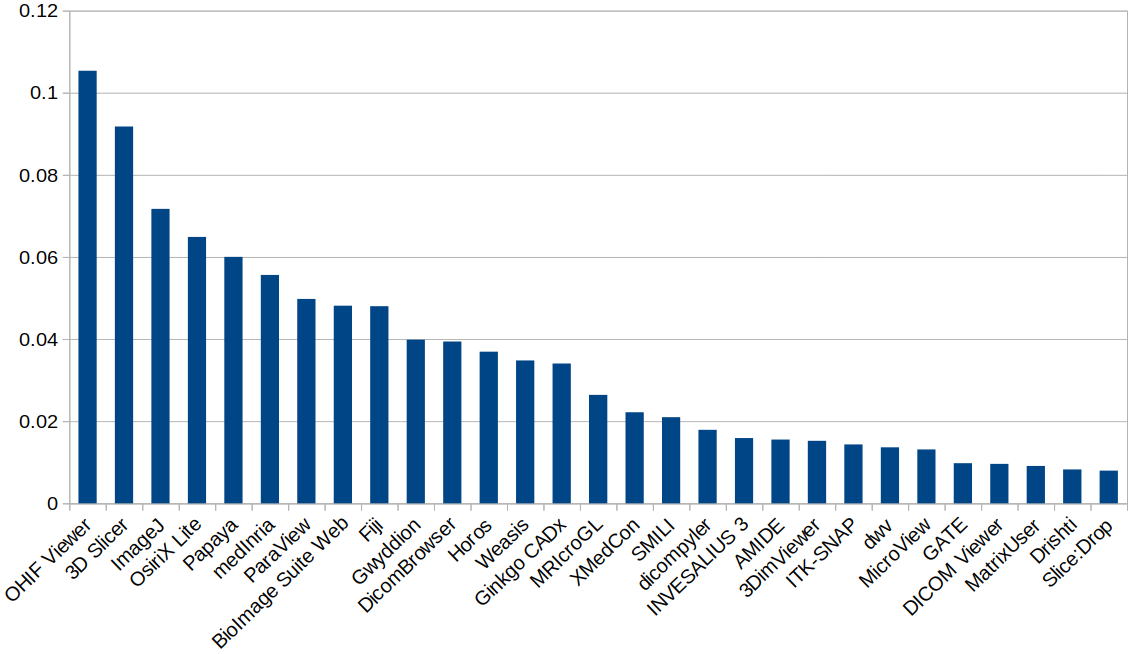
\includegraphics[scale=0.38]{figures/correctness_verifiability_scores.png}
\caption{AHP correctness \& verifiability scores}
\label{fg_correctness_erifiability_scores}
\end{figure}

After examining the source code, we could not find any evidence of unit testing in more than half of the projects. Unit testing benefits most parts of the software's life cycle, such as designing, coding, debugging, and optimization \cite{Hamill2004}. It can reveal the bugs at an earlier stage of the development process, and the absence of unit testing may cause worse \textit{correctness \& verifiability}.

We could not find requirements specifications for most projects. The only document we found is a road map of \textit{3D Slicer}, which contained design requirements for the following changes. However, it did not record the conditions for previous versions. We also could not identify the theory manuals for all of the projects. It seems that even for some projects with well-organized documents, requirements specifications and theory manuals were still missing.

We identified five projects using CI/CD tools, which are \textit{3D Slicer}, \textit{ImageJ
}, \textit{Fiji}, \textit{dwv}, and \textit{OHIF Viewer}.

\section{Surface Reliability}
As described in Section \ref{sec_result_installability}, we could not build \textit{dwv} and \textit{GATE}. However, since there was an online or VM version of them, successful deployment is possible. So the failure of installation did not affect their scores in \textit{surface reliability}. Figure \ref{fg_reliability_scores} shows the AHP results.

\begin{figure}[H]
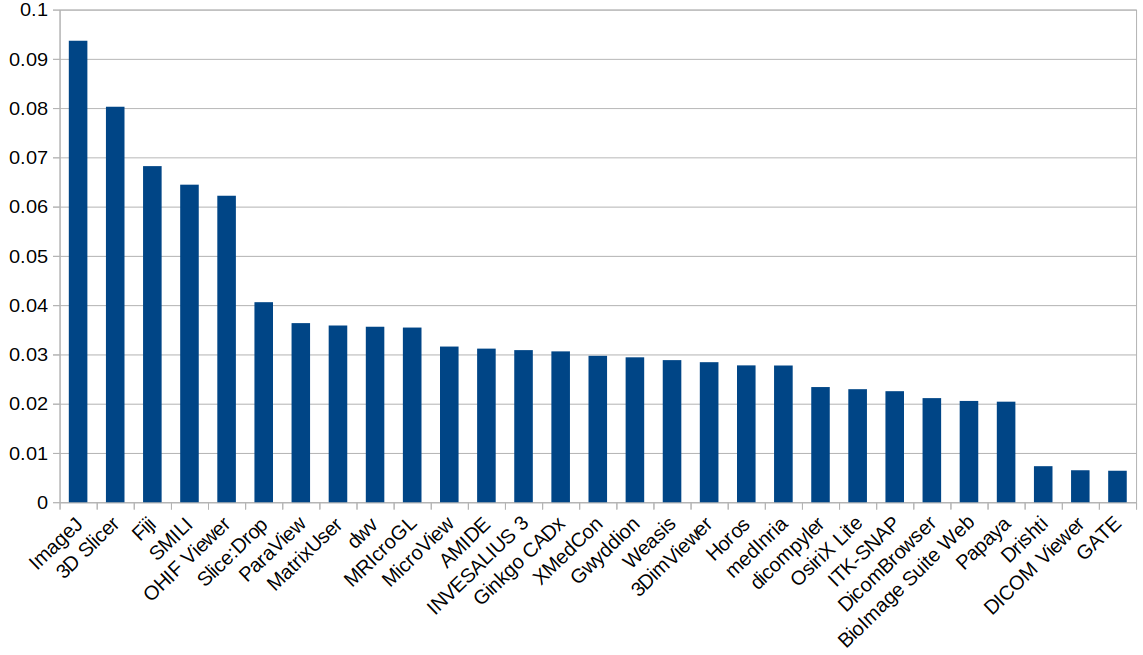
\includegraphics[scale=0.38]{figures/reliability_scores.png}
\caption{AHP surface reliability scores}
\label{fg_reliability_scores}
\end{figure}

When applying basic operations with the software packages, we found out that \textit{Drishti} crashed during loading damaged image files, and \textit{GATE} could not open macro files and lost response several times.

\section{Surface Robustness}
\label{sec_result_robustness}
Figure \ref{fg_robustness_scores} presents the scores for \textit{surface robustness}.

\begin{figure}[H]
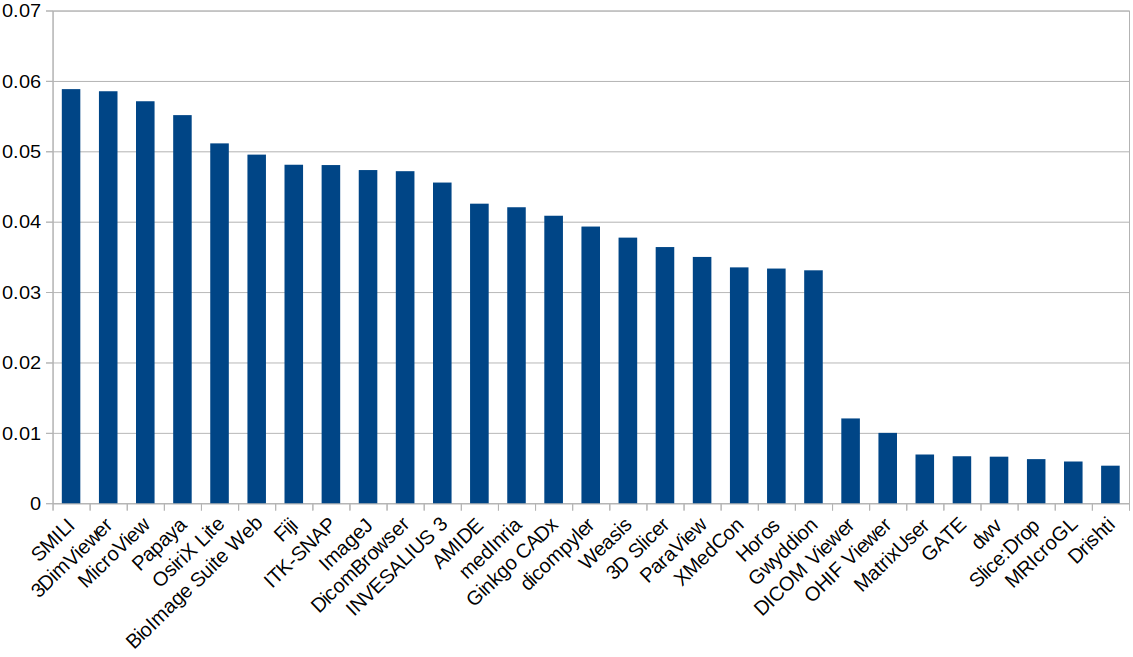
\includegraphics[scale=0.38]{figures/robustness_scores.png}
\caption{AHP surface robustness scores}
\label{fg_robustness_scores}
\end{figure}

The packages with higher scores elegantly handled the unexpected/unanticipated inputs, normally showing a clear error message. We might underestimate the score of \textit{OHIF Viewer} since we needed further customization to load data, and the test was not complete. \textit{MatrixUser}, \textit{dwv}, \textit{Slice:Drop}, and \textit{MRIcroGL} ignored the incorrect format of the input files, and displayed blank or meaningless images. \textit{Drishti} successfully detected the unexpected/unanticipated inputs, but the software crashed as a result. For unknown reasons, \textit{GATE} failed to load both correct and incorrect inputs.

\section{Surface Usability}
Figure \ref{fg_usability_scores} lists the AHP scores for \textit{surface usability}.

\begin{figure}[H]
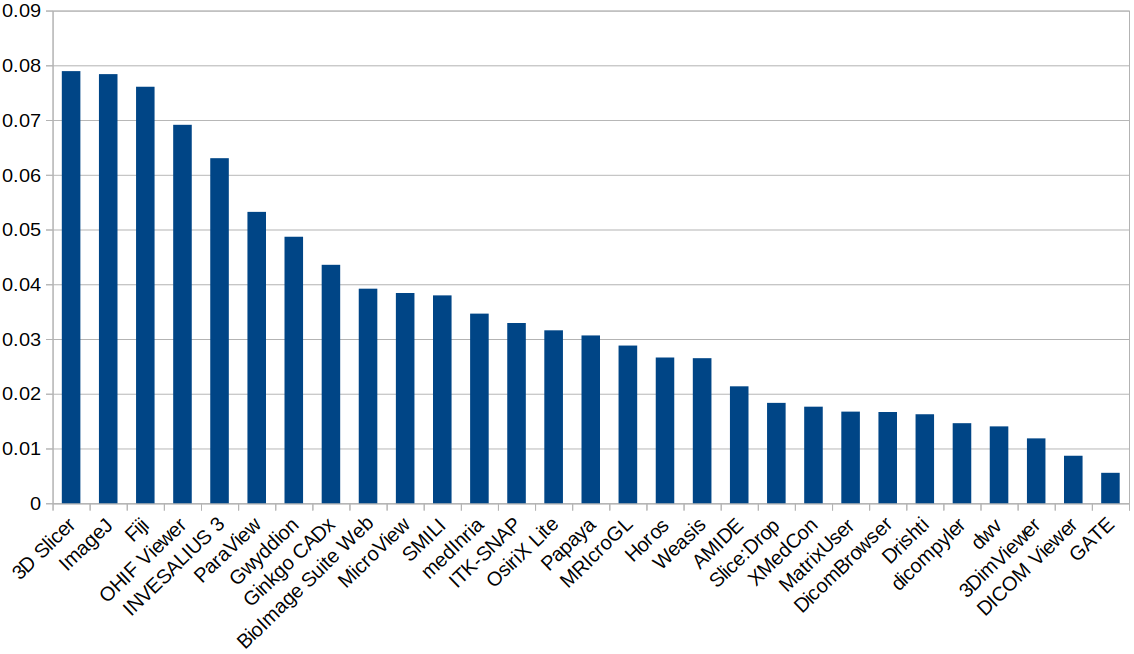
\includegraphics[scale=0.38]{figures/usability_scores.png}
\caption{AHP surface usability scores}
\label{fg_usability_scores}
\end{figure}

We found a getting started tutorial for only 11 projects but a user manual for 22 projects. \textit{MRIcroGL} was the only one with expected user characteristics documented.

The ones with higher scores usually provided both comprehensive document guidance and a good user experience. \textit{INVESALIUS 3} set an excellent example of a detailed and precise user manual. \textit{GATE} also provided a large number of documents, but we think that they conveyed the ideas poorly, as we had trouble understanding and using them.
 
Table \ref{tab_user_support_model} shows the user support models by the number of projects using them. Maybe not every team intended to use GitHub issues to answer users' questions, but many users use them to seek help.

\begin{table}[H]
\centering
\begin{tabular}{ll}
\hline
\multicolumn{1}{c}{User support model} & Number of projects \\ \hline
GitHub issue & 24 \\
GitLab issue, SourceForge discussions & 2 \\
FAQ & 12 \\
Forum & 10 \\
E-mail address & 9 \\
Troubleshooting & 2 \\
Contact form & 1 \\ \hline
\end{tabular}
\caption{\label{tab_user_support_model}User support models by number of projects}
\end{table}

\section{Maintainability}
\label{sec_score_maintainability}
Figure \ref{fg_maintainability_scores} shows the AHP results for \textit{maintainability}. 

\begin{figure}[H]
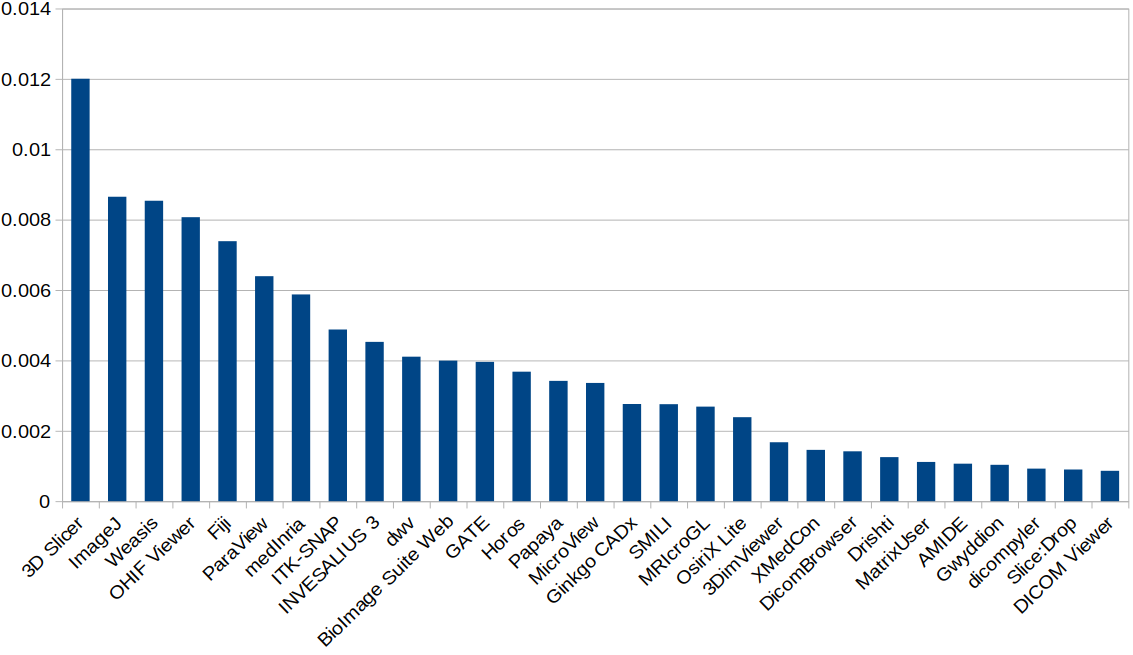
\includegraphics[scale=0.38]{figures/maintainability_scores.png}
\caption{AHP maintainability scores}
\label{fg_maintainability_scores}
\end{figure}

We marked \textit{3D Slicer} with a much higher score than others because it did very well at closing the identified issues, and more importantly, we found it to have the most comprehensive artifacts. For example, as far as we could find out, only a few of the 29 projects had a project plan, developer's manual, or API documentation, and only \textit{3D Slicer}, \textit{ImageJ}, \textit{Fiji} included all three documents. Meanwhile, \textit{3D Slicer} has a much higher percentage of closed issues (91.65\%) than \textit{ImageJ} (52.49\%) and \textit{Fiji} (63.79\%). Table \ref{tab_maintainability_docs} shows which projects had these documents.

\begin{table}[H]
\centering
\begin{tabular}{llll}
\hline
\multicolumn{1}{c}{Software} & Proj plan & Dev manual & API doc \\ \hline
3D Slicer & X & X & X \\
Weasis &  & X &  \\
SMILI &  &  & X \\
ImageJ & X & X & X \\
Fiji & X & X & X \\
dwv &  &  & X \\
BioImage Suite Web &  & X &  \\
OHIF Viewer &  & X & X \\
ParaView & X &  &  \\
INVESALIUS 3 & X &  &  \\
medInria &  & X &  \\
Gwyddion &  & X & X \\ \hline
\end{tabular}
\caption{\label{tab_maintainability_docs}Software with the maintainability documents}
\end{table}

27 of the 29 projects used git as the version control tool; \textit{AMIDE} used Mercurial; \textit{Gwyddion} used Subversion. 24 projects used GitHub for their repositories; \textit{XMedCon
}, \textit{AMIDE}, and \textit{Gwyddion} used SourceForge; \textit{DicomBrowser} and \textit{3DimViewer} used BitBucket.

\section{Reusability}
Figure 4.7 shows the AHP results for \textit{reusability}.

\begin{figure}[H]
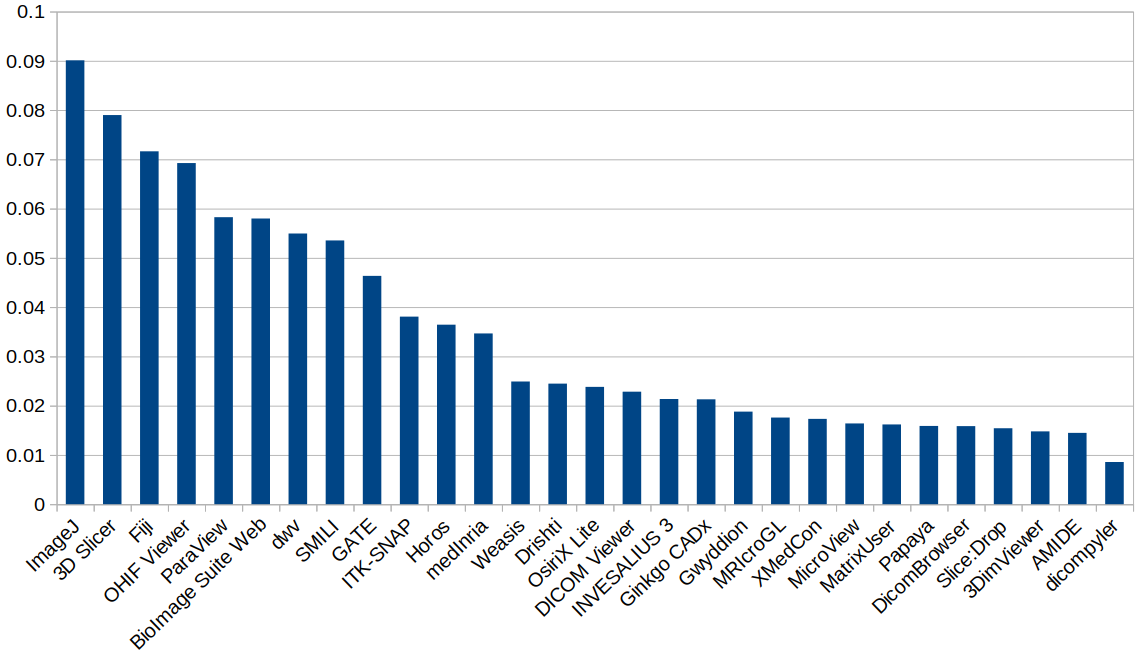
\includegraphics[scale=0.38]{figures/reusability_scores.png}
\caption{AHP reusability scores}
\label{fg_reusability_scores}
\end{figure}

As described in Section \ref{sec_grading_template}, we gave higher scores to the projects with an API document and more code files. As shown in Table \ref{tab_maintainability_docs}, seven projects had API documents. Figure \ref{fg_num_text_files} shows the number of text-based files by projects.

\begin{figure}[H]
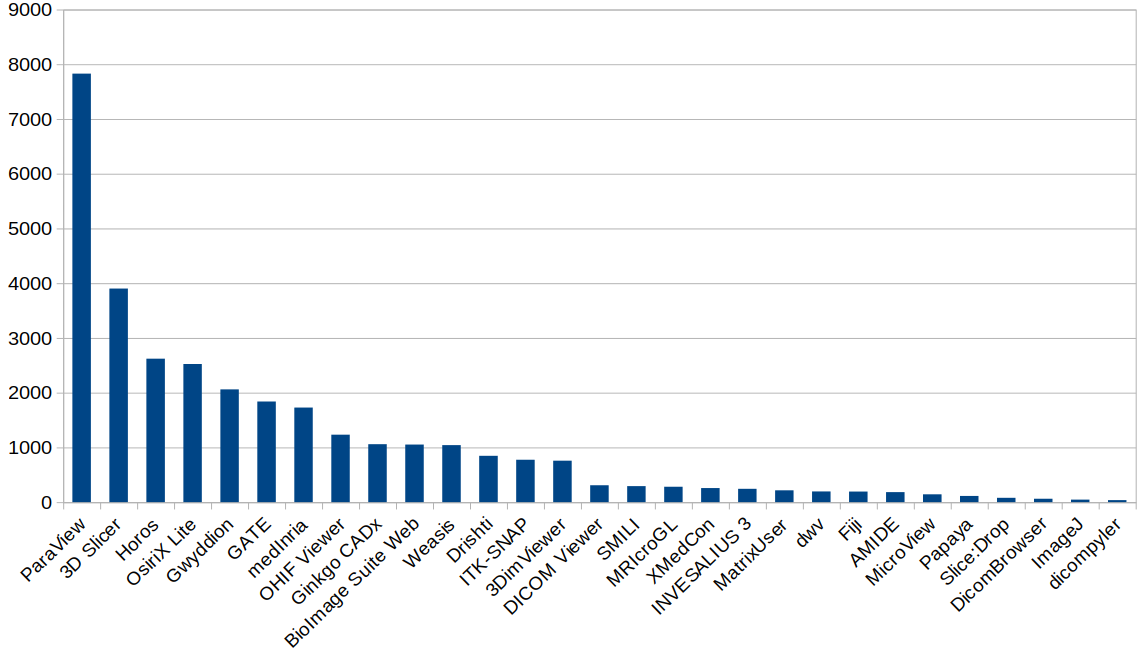
\includegraphics[scale=0.38]{figures/num_text_files.png}
\caption{Number of text-based files files by projects}
\label{fg_num_text_files}
\end{figure}

\section{Surface Understandability}
Figure \ref{fg_surface_understandability_scores} shows the scores for \textit{surface understandability}.

\begin{figure}[H]
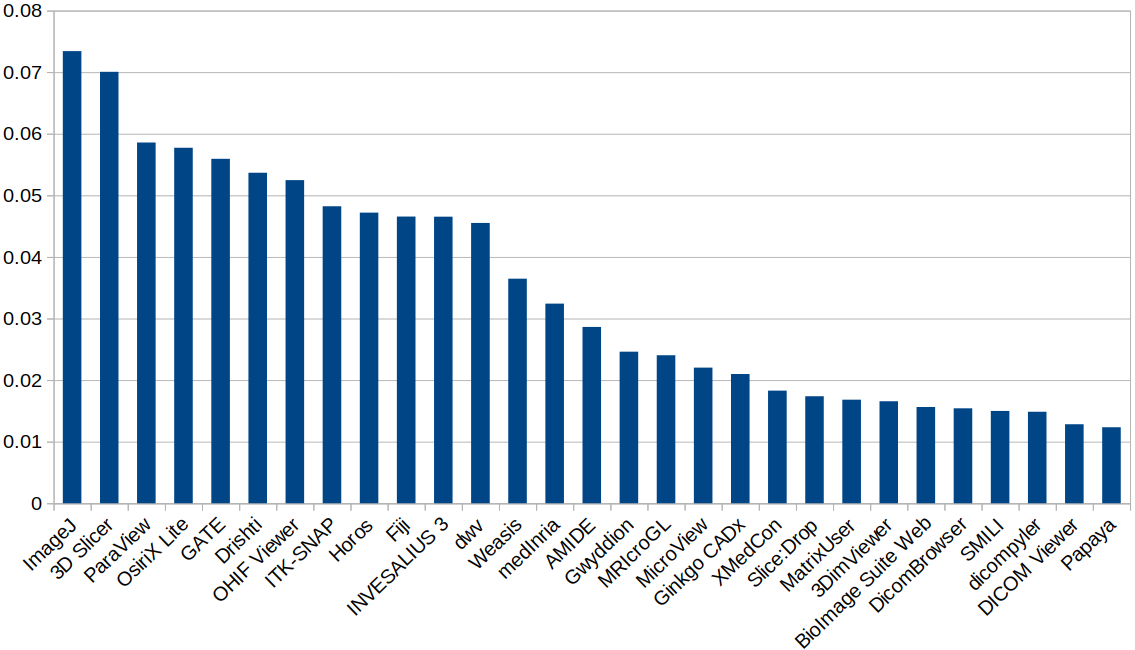
\includegraphics[scale=0.38]{figures/understandability_scores.png}
\caption{AHP surface understandability scores}
\label{fg_surface_understandability_scores}
\end{figure}

All projects had a consistent code style with parameters in the same order for all functions; the code was modularized; the comments were clear, indicating what is being done, not how. However, we only found explicit identification of a coding standard for only 3 out of the 29, which are \textit{3D Slicer}, \textit{Weasis}, and \textit{ImageJ}. We also found hard-coded constants in \textit{medInria}, \textit{dicompyler}, \textit{MicroView}, and \textit{Papaya}. We did not find any reference to the used algorithms in projects \textit{XMedCon}, \textit{DicomBrowser}, \textit{3DimViewer}, \textit{BioImage Suite Web}, \textit{Slice:Drop}, \textit{MatrixUser}, \textit{DICOM Viewer}, \textit{dicompyler}, and \textit{Papaya}. 

\section{Visibility/Transparency}
Figure \ref{fg_visibility_transparency_scores} shows the AHP scores for \textit{visibility/transparency}. Generally speaking, the teams that actively documented their development process and plans scored higher because they delivered better communication to people outside the team.

\begin{figure}[H]
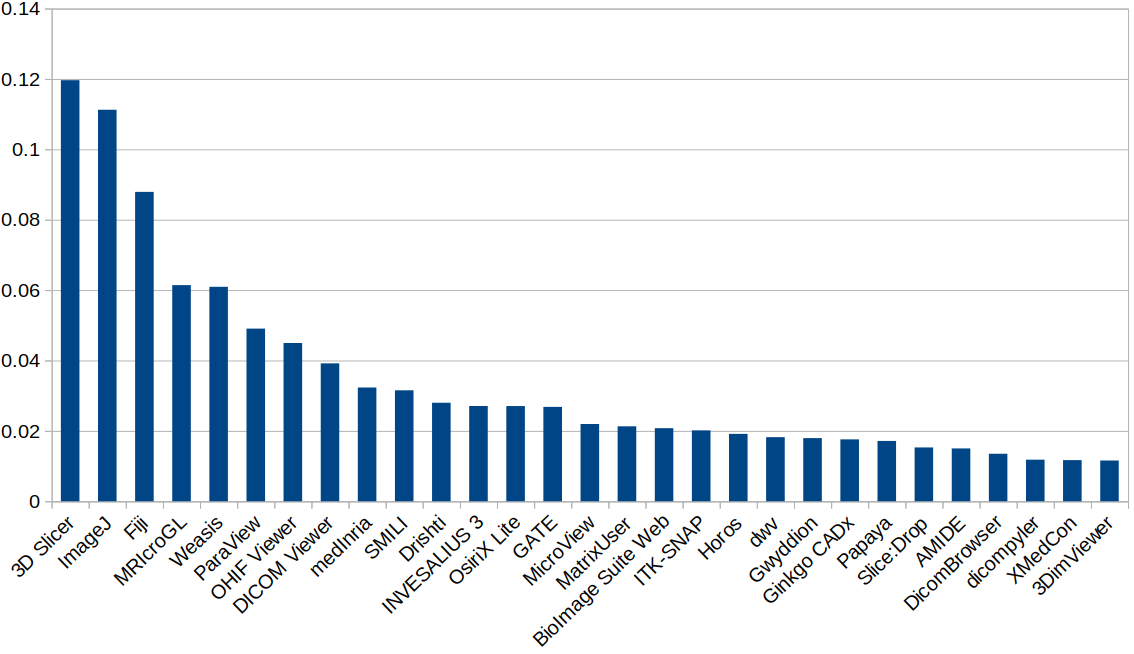
\includegraphics[scale=0.38]{figures/visibility_transparency_scores.png}
\caption{AHP visibility/transparency scores}
\label{fg_visibility_transparency_scores}
\end{figure}

Table \ref{tab_Visibility/Transparency_docs} shows the projects which had documents for the development process, project status, development environment, and release notes.

\begin{table}[]
\centering
\begin{tabular}{lllll}
\hline
Software & Dev process & Proj status & Dev env & Rls notes \\ \hline
3D Slicer & X & X & X & X \\
Weasis \cite{Roduit2021} &  &  & X & X \\
MRIcroGL \cite{Rorden2021} &  &  &  & X \\
SMILI \cite{Chandra2018} &  &  &  & X \\
ImageJ \cite{Rueden2017} & X & X & X & X \\
Fiji \cite{Schindelin2012} & X & X & X &  \\
Horos \cite{horosproject2020} &  &  &  & X \\
OsiriX Lite \cite{PixmeoSARL2019} &  &  &  & X \\
dwv \cite{Martelli2021} &  &  &  & X \\
Drishti \cite{Limaye2012} &  &  &  & X \\
\begin{tabular}[c]{@{}l@{}}BioImage Suite\\ Web\end{tabular} &  &  & X &  \\
OHIF Viewer \cite{Ziegler2020} &  &  & X & X \\
GATE \cite{Jan2004} &  &  &  & X \\
ITK-SNAP \cite{Yushkevich2006} &  &  &  & X \\
ParaView \cite{Ahrens2005} &  & X &  &  \\
MatrixUser \cite{Liu2016} &  &  &  & X \\
DICOM Viewer \cite{Afsar2021} &  &  & X & X \\
INVESALIUS 3 \cite{Amorim2015} &  &  &  & X \\
medInria \cite{Fillard2012} &  &  & X & X \\
MicroView \cite{ParallaxInnovations2020} &  &  &  & X \\
Gwyddion \cite{Nevcas2012} &  &  &  & X \\ \hline
\end{tabular}
\caption{\label{tab_Visibility/Transparency_docs}Software with the visibility/transparency documents}
\end{table}

\section{Overall Scores}

As described in Section \ref{sec_AHP}, for our AHP measurements, there are nine criteria which are the nine software qualities and 29 software packages as the alternatives. We decided to make all nine qualities equally important, so the score of each quality affects the overall scores on the same scale.

Figure \ref{fg_overall_scores} shows the overall scores of all 29 software packages in descending order. Since we produced the scores from the AHP process, the total sum of the 29 scores is precisely 1.

\begin{figure}[H]
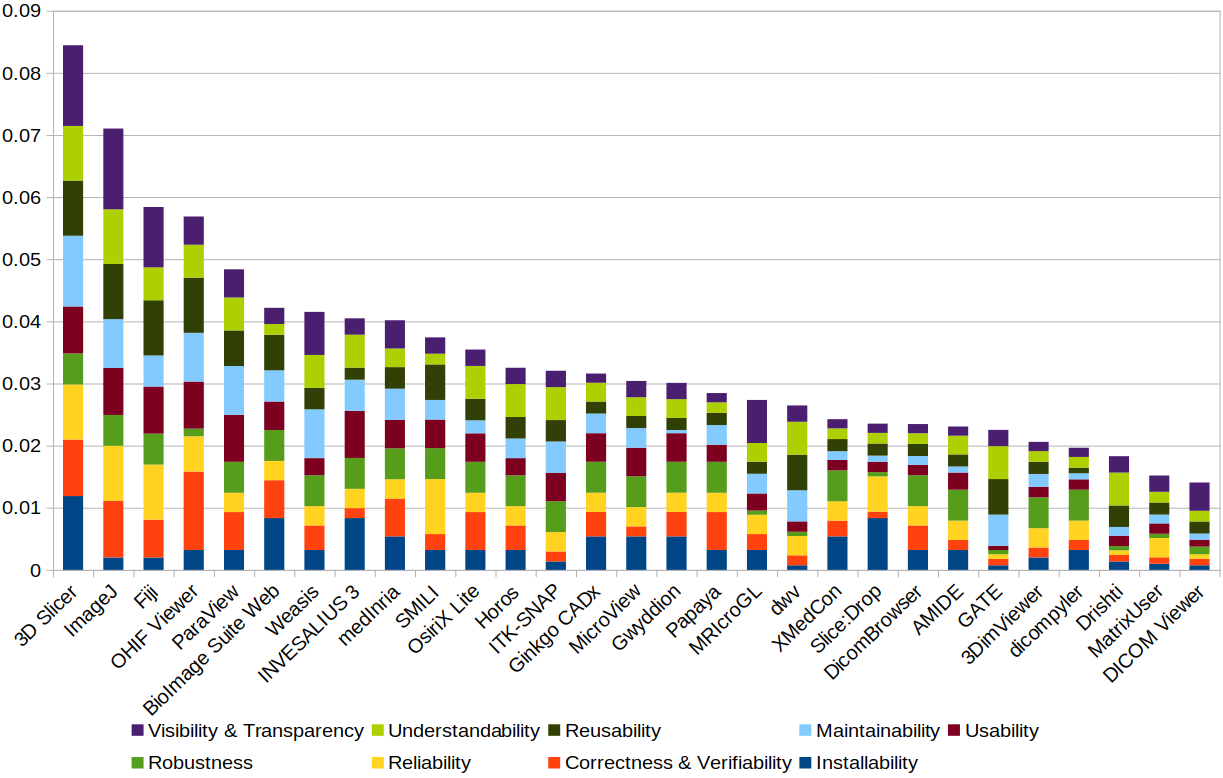
\includegraphics[scale=0.38]{figures/overall_scores.png}
\caption{Overall AHP scores for all 9 software qualities}

\label{fg_overall_scores}
\end{figure}

The top three software products \textit{3D Slicer}, \textit{ImageJ}, and \textit{OHIF Viewer} had higher scores in most criteria. \textit{3D Slicer} ranked in the top two software products for all qualities except \textit{surface robustness}; \textit{ImageJ} ranked in the top three products for \textit{correctness \& verifiability}, \textit{surface reliability}, \textit{surface usability}, \textit{maintainability}, \textit{ surface understandability}, and \textit{visibility/transparency}; \textit{OHIF Viewer} ranked in the top five products for \textit{correctness \& verifiability}, \textit{surface reliability}, \textit{surface usability}, \textit{maintainability}, and \textit{reusability}. We might underestimate its scores of qualities \textit{surface reliability} and \textit{surface robustness} for \textit{DICOM Viewer}, but equally compared it with the other software for the rest seven qualities.
